\documentclass[acmtog]{acmart}
\usepackage{graphicx}
\usepackage{subfigure}
\usepackage{natbib}
\usepackage{listings}
\usepackage{bm}
\usepackage{amsmath}

\definecolor{blve}{rgb}{0.3372549 , 0.61176471, 0.83921569}
\definecolor{gr33n}{rgb}{0.29019608, 0.7372549, 0.64705882}
\makeatletter
\lst@InstallKeywords k{class}{classstyle}\slshape{classstyle}{}ld
\makeatother
\lstset{language=C++,
	basicstyle=\ttfamily,
	keywordstyle=\color{blve}\ttfamily,
	stringstyle=\color{red}\ttfamily,
	commentstyle=\color{magenta}\ttfamily,
	morecomment=[l][\color{magenta}]{\#},
	classstyle = \bfseries\color{gr33n}, 
	tabsize=2
}
\lstset{basicstyle=\ttfamily}

% Title portion
\title{Final Project:\\ {Water Wave Simulation}} 

\author{Name:\quad Yifan Qin Yan Zeng \\ student number:\ 2020533005 2020533182
\\email:\quad qinyf1@shanghaitech.edu.cn zengyan@shanghaitech.edu.cn}


% Document starts
\begin{document}
\maketitle
\begin{abstract}
The water wave simulation 
\end{abstract}

\vspace*{2 ex}

\section{Introduction}
In this project, the following tasks have been done:
\begin{itemize}
    \item Water wave simulation by wave particles algorithm.
    \item Fluid Object interaction in the water with the wave particles algorithm.
\end{itemize}
All things have been done following the instructions and the implementations of the work from ~\cite{yuksel2007wave}. 
The implementation is based on the framework of Assignment 5 (Cloth Simulation).

\section{Previous Work}
This final project is mainly about the realization and the repetition of the work from Yuksel et al.~\cite{yuksel2007wave} 
So in this part, the work that has been done by Yuksel et al. will be briefly introduced. 
In the previous work, they presented a new method for the real-time simulation of the fluid surface waves and the interactions between the waves and the objects. 
They achieved real-time simulation by introducing the concept of water wave particles, which enables a fast and stable way to simulate water. 
With the help of the water wave particles, not only the horizontal water waveform can be simulated, but the vertical water waveform can be simulated. 
Some water wave actions, such as the damping of the water wave and the dispersion of the water waves can also be simulated by using the water wave particles. 

In the previous work, the interactions between the water wave and the object are also simulated. 
In this previous work, they have divided the interactions into two parts. 
One is about the interaction from the object to the water wave, the other one is about the interaction from the water wave to the object. 
For the interaction from the object to the water wave, the object can move horizontally and vertically. 
No matter what direction the object moves, as long as the object interacts with the water, the object can generate waves by generating the water wave particles. 
And for the interaction from the water wave to the object. 
The object will not only have the buoyant force, which is calculated with the volume that the object inside the fluid and the density of the fluid medium. 
The buoyant force is mainly used to cancel out the effect of gravity. 
The water wave will also have forces on the object, such as the drag force and the lift force, which are used to change the movement of the object in the water. 

As this project is the realization and the repetition of the work, all the things that are depicted above will be introduced again in the following parts. 
And more details will also be introduced in the following parts. 

\section{Implementation Details}
\subsection{Water Wave Simulation}
This part will introduce how we implement the wave particles algorithm to solve the wave equation and simulate the water wave.
The core algorithm of our project was implemented in file 'water-surface.h' and 'water-surface.cpp', which include a class called \verb|WaterSurface| and a struct called \verb|WaterParticle|.

For \verb|WaterSurface|, it has the member variables that store all water particles, and other variables that define the coefficients that can represent the characteristics of a water surface, like the water density, wave speed, lift coefficient and drag coefficient, the details of these coefficients will be introduced later.
The member functions of \verb|WaterSurface| include the local-world transformation function and the simulation function, the most important functions are the functions in the simulation pipeline, each time step, the main procedures including:
\begin{enumerate}
    \item \verb|IterateWaveParticles()| 
    \item \verb|ComputeObjectForces()| 
    \item \verb|IterateObject()| 
    \item \verb|GenerateWaveParticles()| 
    \item \verb|RenderHeightFields()|
\end{enumerate}
The implementations of each function will be introduced later. 

For \verb|WaterParticle|, it has the member variables that describe a water particle, including amplitude, radius, dispersion angle, surviving time, position, propagate direction and horizontal direction, that cover all the information needed in the simulation procedure.

Now we will introduce the implementation of the functions above to help readers to understand our project.
\subsubsection{Iterate Wave Particles}
This function will update the positions of all water particles and handle the subdivision and reflection events of every water particle.

First and foremost, we need to check manually whether the amplitude of the particle is low by comparing the amplitude of the particle with a threshold. 
The comparison is based on the condition which is $a < threshold$, where $a$ is the amplitude of the particle and $threshold$ is a hyper-parameter that can be tuned to control the life span and the visual effect of the wave particles. 
If the condition ($a < threshold$) holds, then the particle is just eliminated in all the particles. 
If the condition does not hold, it means that the particle still survives. 


Secondly, the propagate distance of every water particle will be calculated by the equation: $d_{prop} = t_{s} * v_{wave}$, where $t_{s}$ is the surviving time (time period the water particle exists) and $v_{wave}$ is the wave speed specified by the water surface. 
The reason why we need the distance that the particle has propagated is that the product of the propagation distance $d_{prop}$ and the dispersion angle $r_{disp}$ represents the length of the arc that the water particle controls. 
On the other hand, the product of the propagation distance $d_{prop}$ and the dispersion angle $r_{disp}$ also indicates the distance from this wave particle to other wave particles. 
So the product can be used as an indicator of whether the particle needs to be subdivided or not. 

If the subdivision condition ($d_{prop}\cdot r_{disp} > c \cdot R$ where $r_{disp}$ is the radians of dispersion angle, $R$ is the particle radius and $c$ is a human-defined constant) holds, the particle should be subdivided to three particles, in our implementation, each particle will carry the information of three particles, one is itself and the other two are 'future' particles that when the current particle is subdivided, the two new-generated particles will directly use the position and direction value and that store in the original's particle. 
When creating a new water particle (the implementation is in function \verb|create_particle|), the position of the real particle and two 'future' particles will be the same, all three positions are get from the particle that is subdivided. 
The propagation direction of the real particle is directly inherited from the original particle that is subdivided. 
And the propagation direction of the two 'future' particles will be calculated by dividing the dispersion angle into three parts and getting the other two directions. 
All the horizontal directions will be the cross productions of propagation directions and the up directions.

After handling the subdivision events, we should update the attributes of all water particles (including the newly generated ones). 

For amplitude, it will exponentially decay to limit the number of particles that exists. 
Originally, the damping coefficient is set as a constant value. 
However, we found that this setting of the damping coefficient is not ideal because we want the damping of the amplitudes of the particles to be stronger when there are too many particles in the scene and the damping of the particles should be relatively smaller when there are few particles in the scene. 
In order to achieve this kind of effect, the setting of the damping coefficient in another work was used. 
Based on the work~\cite{jeschke2017water}, the setting of the damping coefficient follows the following equation: 
\begin{equation*}
    a \leftarrow a e^{-\alpha \Delta t}
\end{equation*}
where $a$ represents for the amplitude of the particles and the $\Delta t$ is the time for simulation delta time.
$\alpha$ is calculated by another equation, where the number of the wave particles takes the effect, and the calculation of $\alpha$ is given by 
\begin{equation*}
    \alpha = 1 + \beta \max(0, N / N_{max} - 1)^2
\end{equation*}
where $N$ indicates the current number of wave particles and $N_{max}$ is a hyper-parameter that can be set to control the upper bound of the number of the wave particles. 
In other words, if the number of wave particles exceeds the upper bound of the number of the wave particles $N_{max}$, a stronger damping will take effect. 
In the equation, $\beta$ is also a hyper-parameter that can be tuned to control the damping when the number of wave particles is too large. 
And in the work \cite{jeschke2017water}, they see $\beta$ as a stiffness coefficient. 
Here we follow the implementation in the previous work and set the hyper-parameter $\beta$ as $100$. 

For particle surviving time, it will be increased by simulation delta time. 
For positions of three particles, the update equation is $p_{new}=p_{old}+v_{wave}\cdot \Delta t * d_{prop}$, where $p_{new},p_{old}$ are new position and old position, $\Delta t$ is the simulation delta time and $v_{wave}$ is wave speed (scalar) that is constant for wave particles algorithm.

Then the reflection events should be handled. 
The reflection events between the water wave and the object will be introduced in the fluid object interaction part. 
Now we discuss the reflection that happened when the water wave reaches the boundary. 
When a water particle hit a boundary, the propagation direction will change, the new direction will be calculated by doing an ideal reflection with the boundary, and the normal vector of the reflection plane will be decided by the boundary the particle hits. 
Then function \verb|glm::reflect| will be called to get the new direction.
\subsubsection{Generate Wave Particles}
This function will generate new wave particles, including the rain drop effects and the water particles generated by fluid-object interaction (introduced in the next section). 
To implement the rain drop effect, a water particle will be created after certain time steps, the position is uniformly sampled from the water surface area. 
Because for the rain drop effect, the initial dispersion angle of the wave particle is $2\pi$, which can also be seen as the whole circle, the propagate direction does not matter in this case. 
So the initial propagate direction of the rain drop water particle can be set as any direction on the plane of the water surface. 

Similar to the instructions in the work~\cite{yuksel2007wave}, the rain drop effect will not only create the wave that causes the height of the water surface to increase, but it will also generate waves that cause the height of the water surface to decrease. 
In order to achieve this kind of effect, we will first generate a wave particle with a positive amplitude at the position of the rain drop, which was randomly and uniformly sampled on the surface. 
Then after a specific time $t$, another wave particle with a negative amplitude will also be generated at the position of the rain drop. 
The time difference $t$ between the wave particle with positive and the wave particle with negative amplitude can be tuned in order to get a better visual effect. 
\subsubsection{Render Height Field}
This function will compute the height field of the water surface using the wave particles algorithm. For a water surface, it will have some water vertices that are uniformly distributed in the water plane. Following the wave particle algorithm ~\cite{yuksel2007wave}, we need to calculate the vertical and horizontal components (see Fig \ref{fig:1}) of each water vertex then we can render the water surface. The vertical component of a water vertex in time step $t$, $\eta_{z}(\mathbf{x},t)$ is calculated by the equations:
\begin{equation*}
   \begin{aligned}
        \eta_{z}(\mathbf{x},t) &= \sum_{i}D_i(\mathbf{x},t) \\
        D_i(\mathbf{x},t) &= \frac{a_i}{2}\left( \cos \left( \frac{\pi |\mathbf{x}-\mathbf{x}_i(t)|}{r_i}\right)+1\right)\Pi\left(\frac{\pi |\mathbf{x}-\mathbf{x}_i(t)|}{2r_i}\right)
    \end{aligned}
\end{equation*}
where $\mathbf{x}$ is the water plane position of water vertex, $D_i(\mathbf{x},t)$ is local deviation function corresponding to particle $i$, $\mathbf{x}_i(t)$ is the position of wave particle $i$ in time step $t$ and $a_{i}$ is the amplitude of the particle $i$ in time step $t$. 
$r_{i}$ is the radius of particle $i$ and $\Pi$ is the rectangle function, and we follow the implementation in ~\cite{yuksel2007wave} that the rectangle function is given by $\Pi(x)$ is $1$ for $|x| < 0.5$, $0.5$ for $|x|=0.5$ and $0$ otherwise.
Similarly, the horizontal component is:
\begin{equation*}
   \begin{aligned}
        \eta_{xy}(\mathbf{x},t) &= \sum_{i}D^L_i(\mathbf{x},t) \\
    \end{aligned}
\end{equation*}
where $D^L_i$ is a longitudinal local deviation function, which can be formulated as
\begin{equation*}
   \begin{aligned}
        D^L_i(\mathbf{x},t) &= L_i(\hat{\mathbf{u}}_i\cdot(\mathbf{x}-\mathbf{x}_i))D_i(\mathbf{x},t)
    \end{aligned}
\end{equation*}
where $\hat{\mathbf{u}}_i$ is the propagation direction of particle $i$ and $L_i$ is a vector function describing the longitudinal waveform
\begin{equation*}
   \begin{aligned}
        L_i(u)=-\sin \left(\frac{\pi u}{r_i} \right) \Pi \left(\frac{u}{2r_i}\right)\hat{\mathbf{u}}_i
    \end{aligned}
\end{equation*}
where $r_{i}$ is the radius of particle $i$.
After calculating the vertical and horizontal components, the positions of water vertices will be updated for further simulation and rendering.
\begin{figure}[!htb]
  \centering
  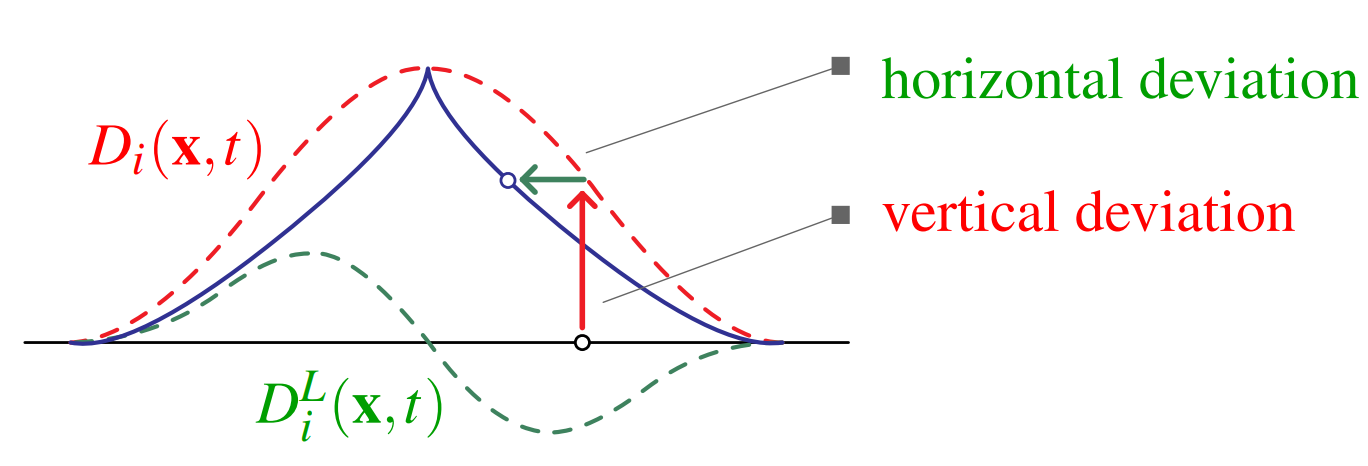
\includegraphics[width=0.4\textwidth]{image/component.png}
  \caption{Components of the local deviation function in 2D} 
\label{fig:1}
\end{figure}
\subsection{Fluid object interaction}
In our project, we implement the water-sphere interaction. For sphere, we have a struct \verb|Sphere| that store the necessary information for simulation, including: center position, radius, radius of the water plane cutting area, acceleration, velocity and local velocity (the sphere velocity in water coordinate that suppose the water is static). 
The interaction cover two parts, fluid to sphere interaction and sphere to fluid interaction. The fluid to sphere interaction is implemented in function \verb|ComputeObjectForces| and \verb|IterateObject| and the sphere to fluid interaction including the reflection and some wave particle generations.
\subsubsection{Compute Object Forces}
 The fluid to sphere force including three component: buoyancy force, drag force and lift force.
 The static component of the force is buoyancy:
 \begin{equation*}
   \begin{aligned}
        \mathbf{F}_{buoyancy} = -\mathbf{g}\rho V_{displaced}
    \end{aligned}
\end{equation*}
where $\mathbf{g}$ is the gravitational acceleration, $\rho$ is the density of the fluid, and $V_{displaced}$ is the volume of the sphere inside the fluid that can be formulated by equation:
 \begin{equation*}
   \begin{aligned}
        V_{displaced} = \pi h^2\left(R-\frac{h}{3}\right)
    \end{aligned}
\end{equation*}
where $R$ is the sphere radius and $h$ is the depth inside.
The dynamic forces are computed over the interface of fluid and object and they are based on the relative motion of the object surface to the fluid. One component of dynamic force is \textit{drag force} that in the opposite direction of relative motion. The other component perpendicular to the relative motion is \textit{lift force}. (See Fig \ref{fig:2})
\begin{figure}[!htb]
  \centering
  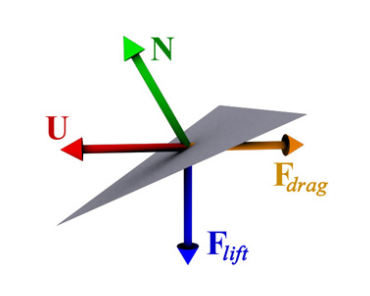
\includegraphics[width=0.3\textwidth]{image/force.png}
  \caption{Directions of drag and lift forces on an object face.} 
\label{fig:2}
\end{figure}
The drag and lift forces acting on each face are:
 \begin{equation*}
   \begin{aligned}
        \mathbf{F}_{drag} &= -\frac{1}{2}\rho C_{D}|A||\mathbf{U}|\mathbf{U} \\
        \mathbf{F}_{lift} &= -\frac{1}{2}\rho C_{L}|A||\mathbf{U}|\left(\mathbf{U} \times \frac{(\mathbf{N} \times \mathbf{U})}{|(\mathbf{N} \times \mathbf{U})|}\right)
    \end{aligned}
\end{equation*}
where $C_D$ and $C_L$ are the drag and lift coefficients, $\mathbf{U}$ is the local velocity, and $A$ is the effective area of the face. 

For the local velocity $\mathbf{U}$, it can also be seen as the relative velocity and it is updated in the part of iterating wave particles. 
As in our implementation, the propagation direction of the water wave particle will change when it bumps into the surfaces of the object, but the original direction of the propagation of the sphere is needed to calculate the local velocity $\mathbf{U}$. 
So for each water wave particle that bumps into the surface of the object, before the change of its propagation direction, the local velocity of the object is subtracted with the propagation velocity of the particle. 
Because the local velocity $\mathbf{U}$ record the velocity of the object in the water coordinate that the water surface is seen as static. 

For the effective area of the surface $A$, only the area of the surface that is inside the fluid will be considered. 
And only the area of the surface that is not only perpendicular to the water surface but also the perpendicular to the local velocity of the object will be considered as the effective area $A$ of the surface. 

For sphere, the effective area depends on the sphere radius $R$ and the relative depth $h$. 
It is needed for the object to generate wave particles caused by the vertical movement of the object. 
When the object is moving vertically due to the effect of the buoyancy force and the gravity, the object will also creates water wave particles. 
Such kinds of water wave particles are implemented following the instructions in the work~\cite{yuksel2007wave}. 
However, the effects of this kinds of water wave particles are too small that it can merely be seen.  
After calculating the three components, the combined acceleration can be derived. Then the velocity can be updated by $v_{new} = v_{old} + a_{all} \Delta t$. 
\subsubsection{Iterate Objects}
This function will handle the sphere-boundary collision and update the sphere position. To handle the collision event, the component of the sphere velocity that parallel to the boundary normal will be set to $0$ when the collision happen.
Then the sphere position will be updated by $p_{new} = p_{old} + v_{sphere} \Delta t$.
\subsubsection{Sphere to fluid interaction}
The sphere to fluid interaction including the reflection when the water wave pass through the sphere and the water particle generation near the sphere. The reflection in sphere surface is handled in \verb|IterateWaveParticles|, the idea is similar to the wave-boundary reflection, the only difference is that the reflection normal is derived by formula $\mathbf{N}_{ref} = normalize(p_{particle} - p_{center})$ where the $p_{particle}$ is the particle position and $p_{center}$ is the sphere center position. After calculating the reflection normal, we can get the new direction by calling \verb|glm::reflect|.
To achieve the sinking and floating effect of the sphere on the water surface, there will be particle generations near the sphere. The full $2\pi$ angle is divided to eight directions as the propagation directions of the new particles, the current position of the eight particles can be derived from $p_{center}$ and the radius on surface, and their amplitude is $a = \frac{1}{2} (d_{prop}\cdot (p_{current}-p_{old})$ where $d_{prop}$ is the one of eight propagation direction and $p_{current},p_{old}$ are the current and old position intersect with water surface in this propagation. The dispersion angle of the generated particles is set to $\pi$ to simulate the realistic reflection results.
\section{Result}
\begin{figure}[H]
    \centering
    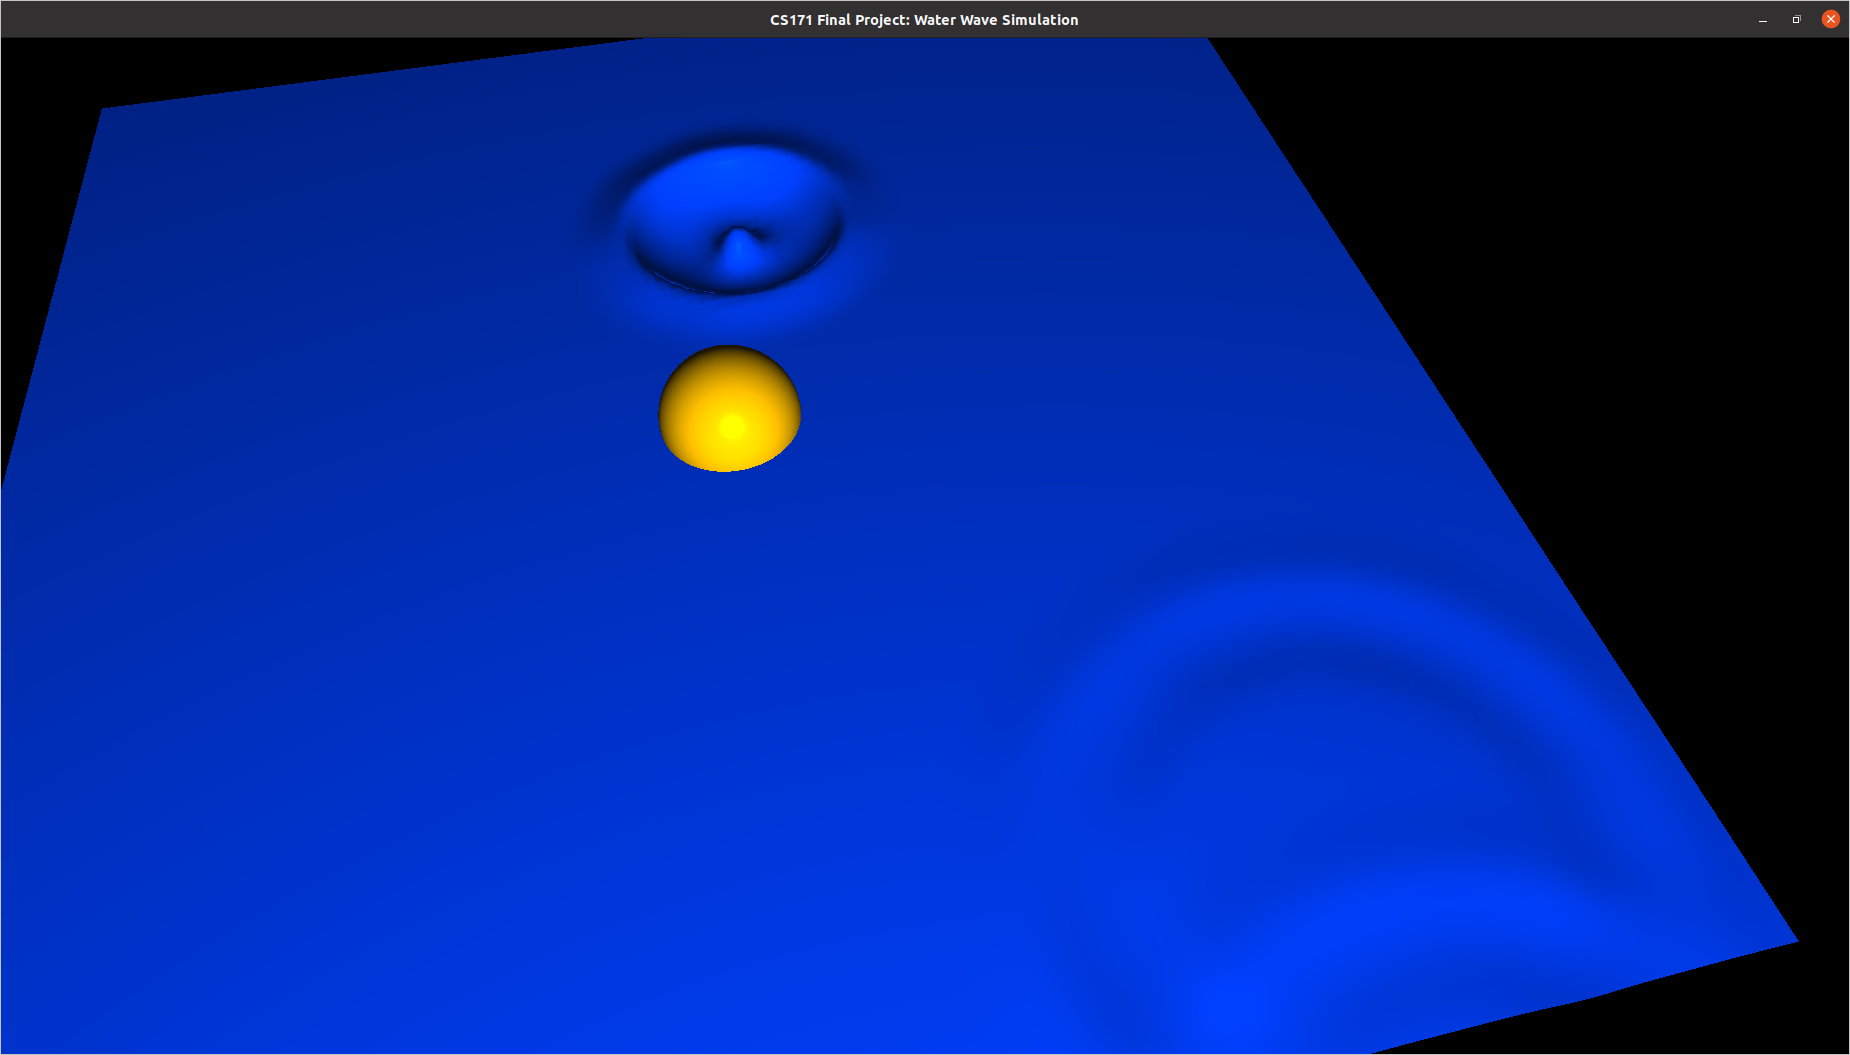
\includegraphics[scale=0.1]{image/Raindrop effect.png}
    \caption{Raindrop effect in water surface.}
\end{figure}
\begin{figure}[H]
    \centering
    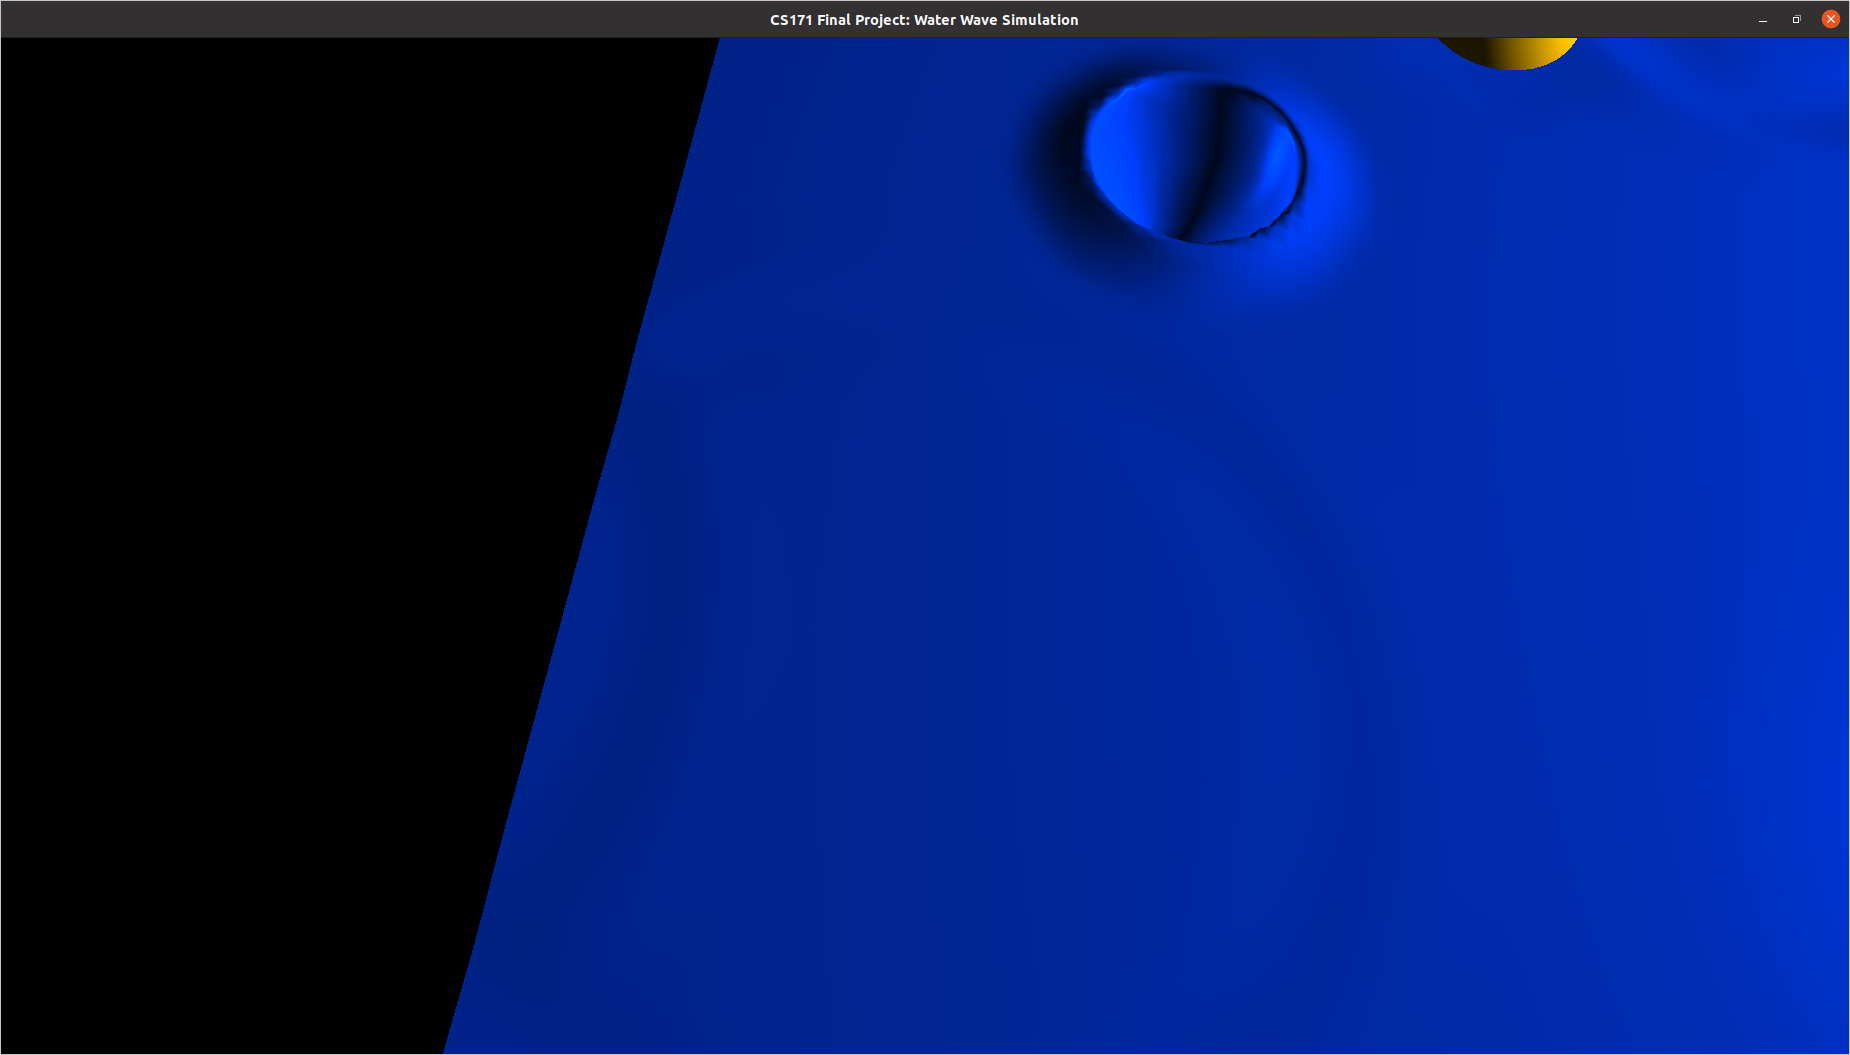
\includegraphics[scale=0.1]{image/Wave reflected by wall.png}
    \caption{Wave reflected by wall.}
\end{figure}
\begin{figure}[H]
    \centering
    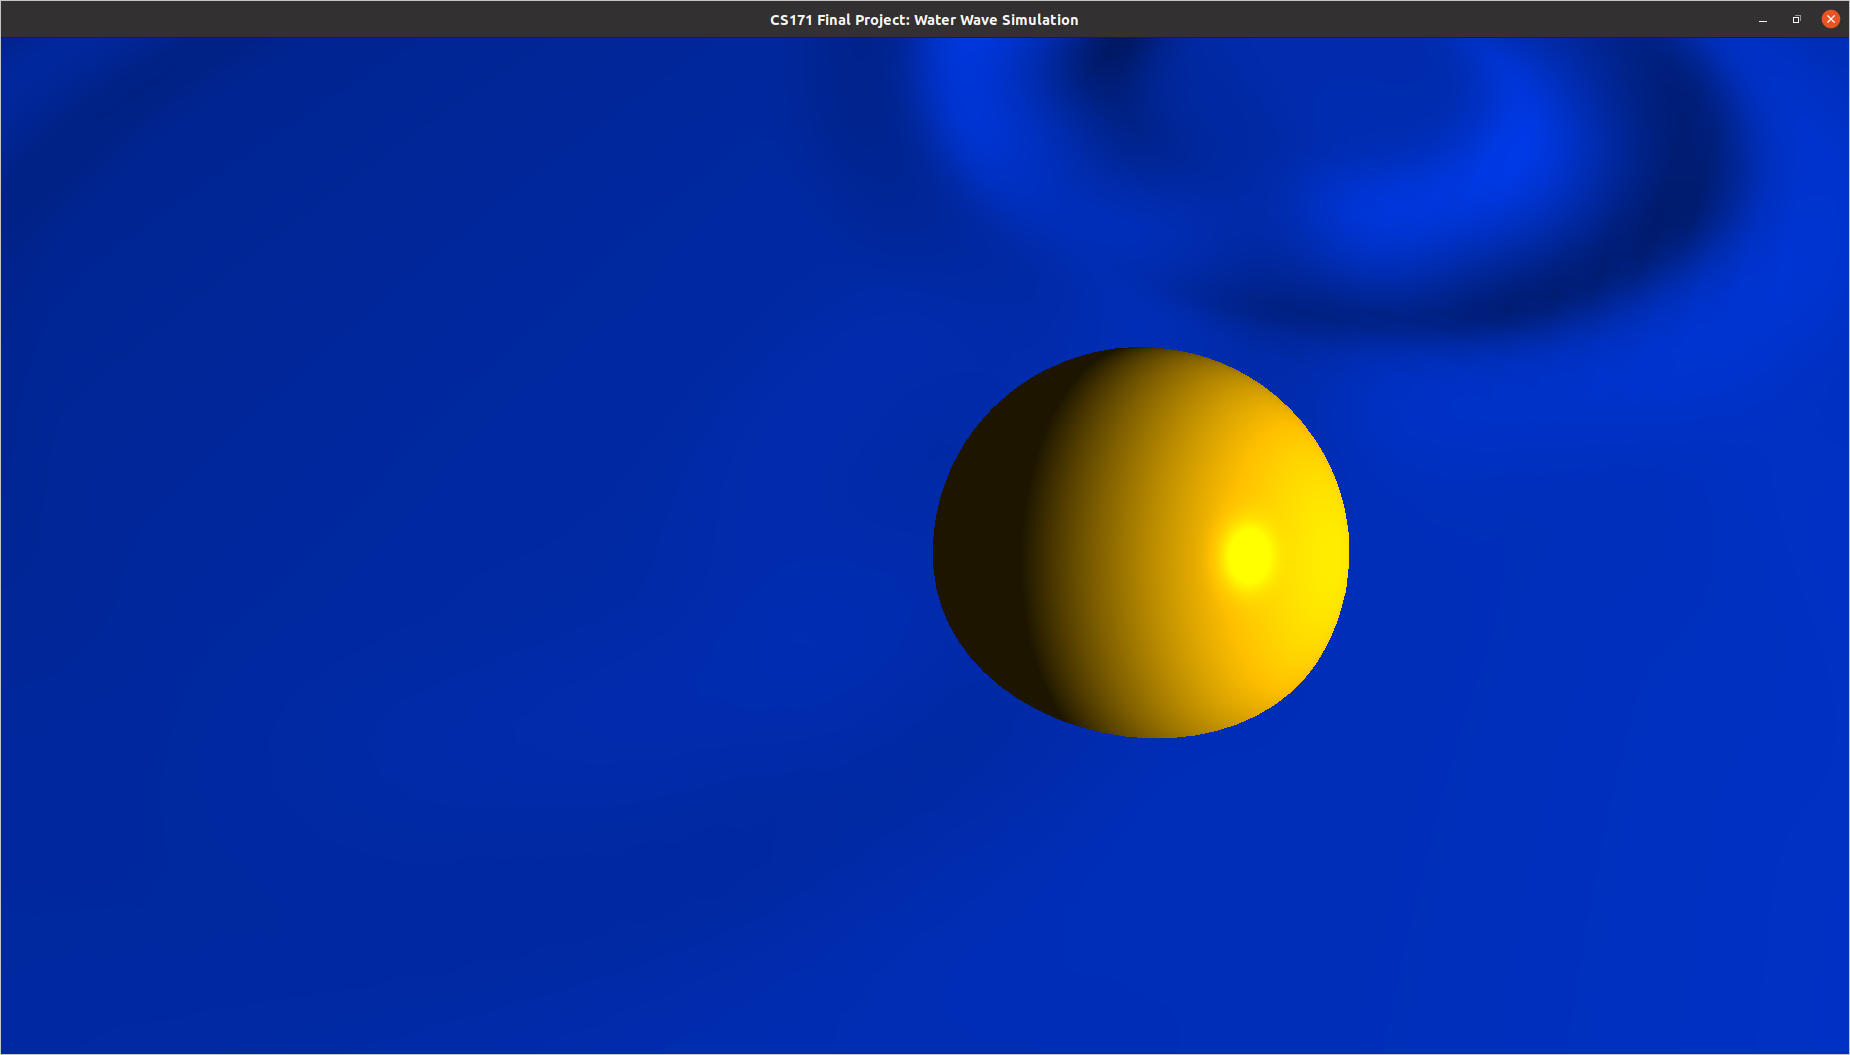
\includegraphics[scale=0.1]{image/Wave reflected by object.png}
    \caption{Wave reflected by object.}
\end{figure}
\begin{figure}[H]
    \centering
    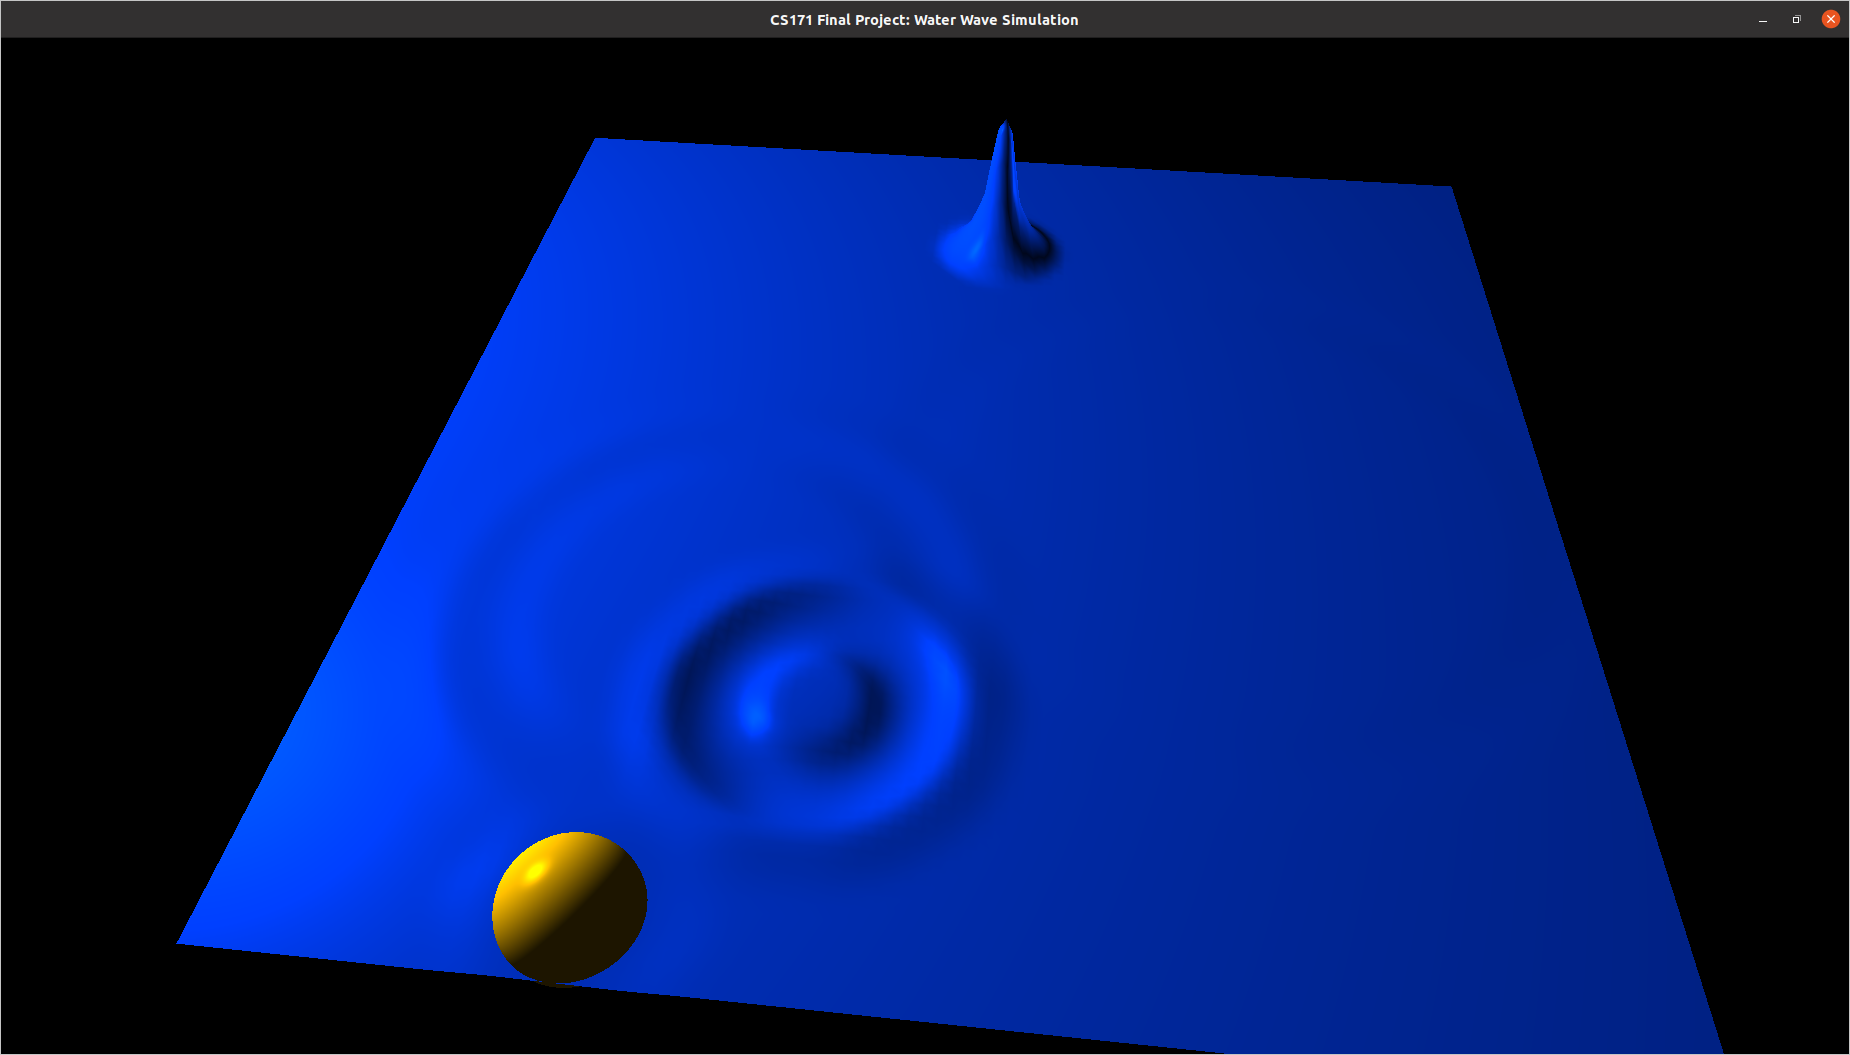
\includegraphics[scale=0.1]{image/Two waves.png}
    \caption{Collision of two waves.}
\end{figure}
\begin{figure}[H]
    \centering
    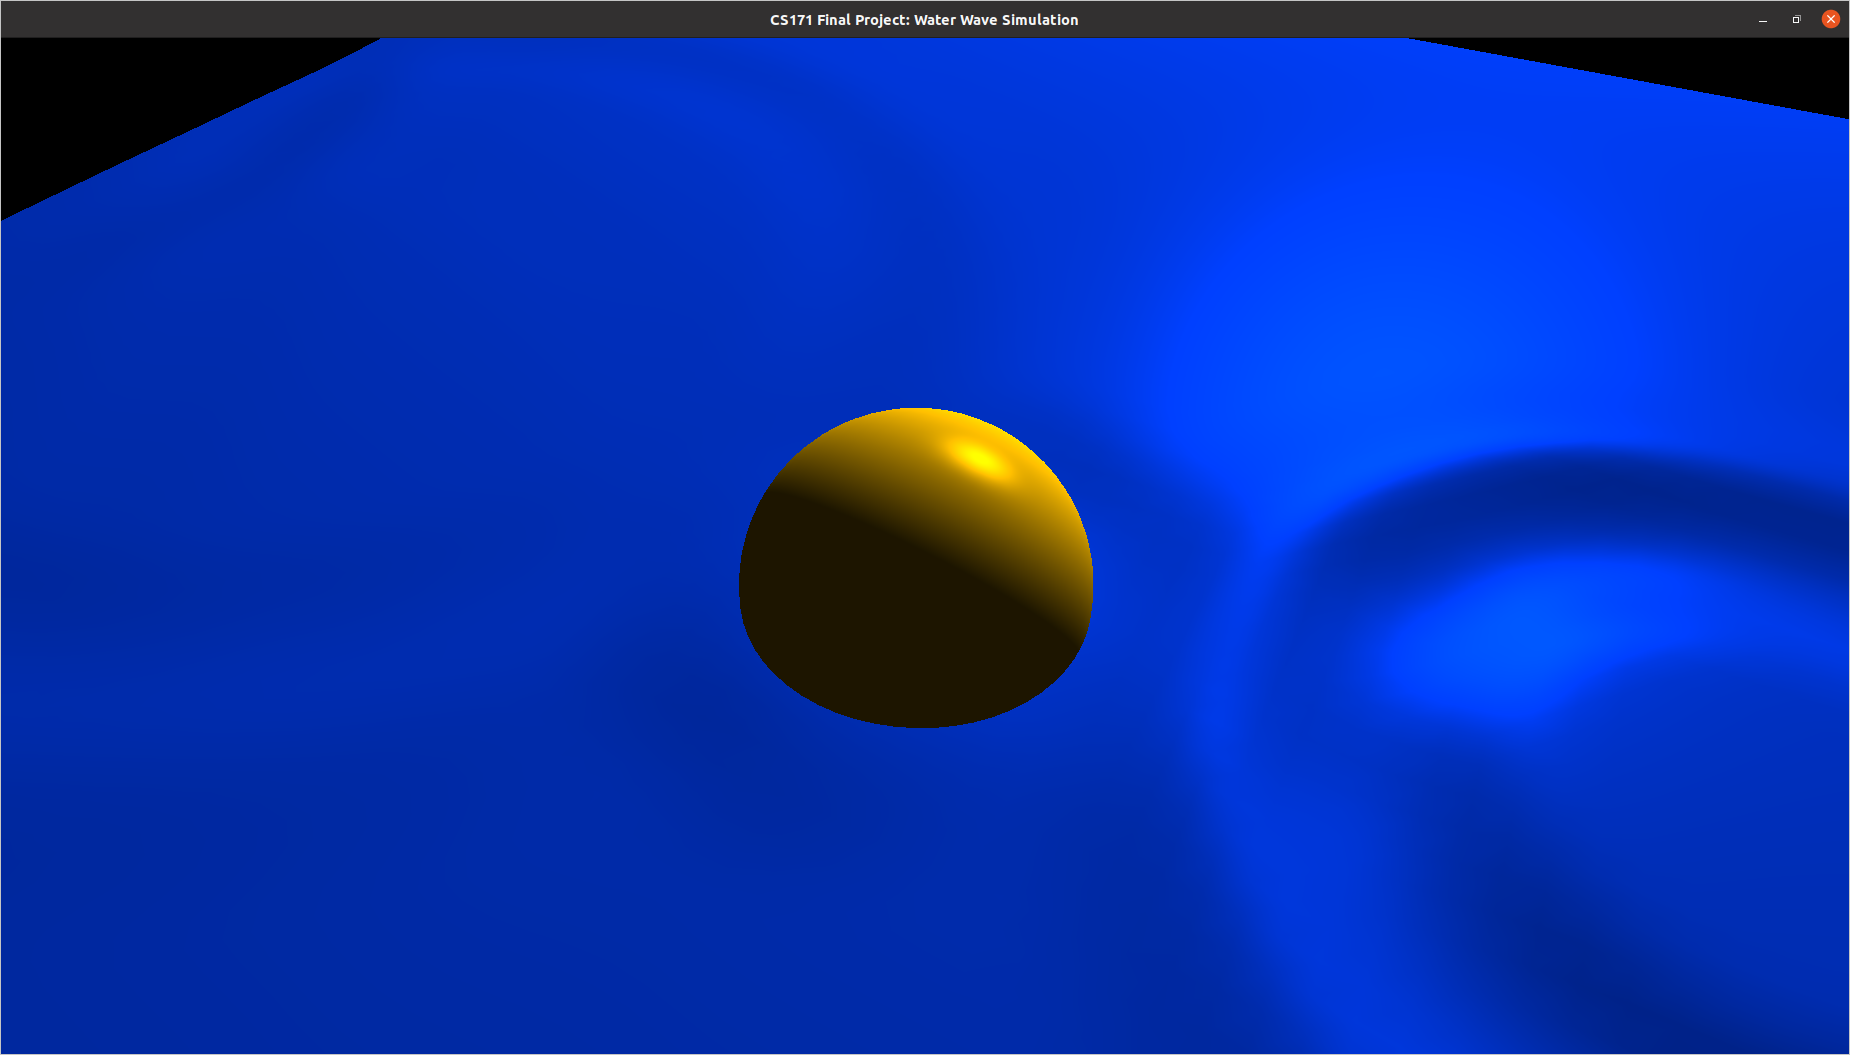
\includegraphics[scale=0.1]{image/Wave created by object.png}
    \caption{Wave created by object.}
\end{figure}
\begin{figure}[H]
	\centering
    \subfigure[]{
		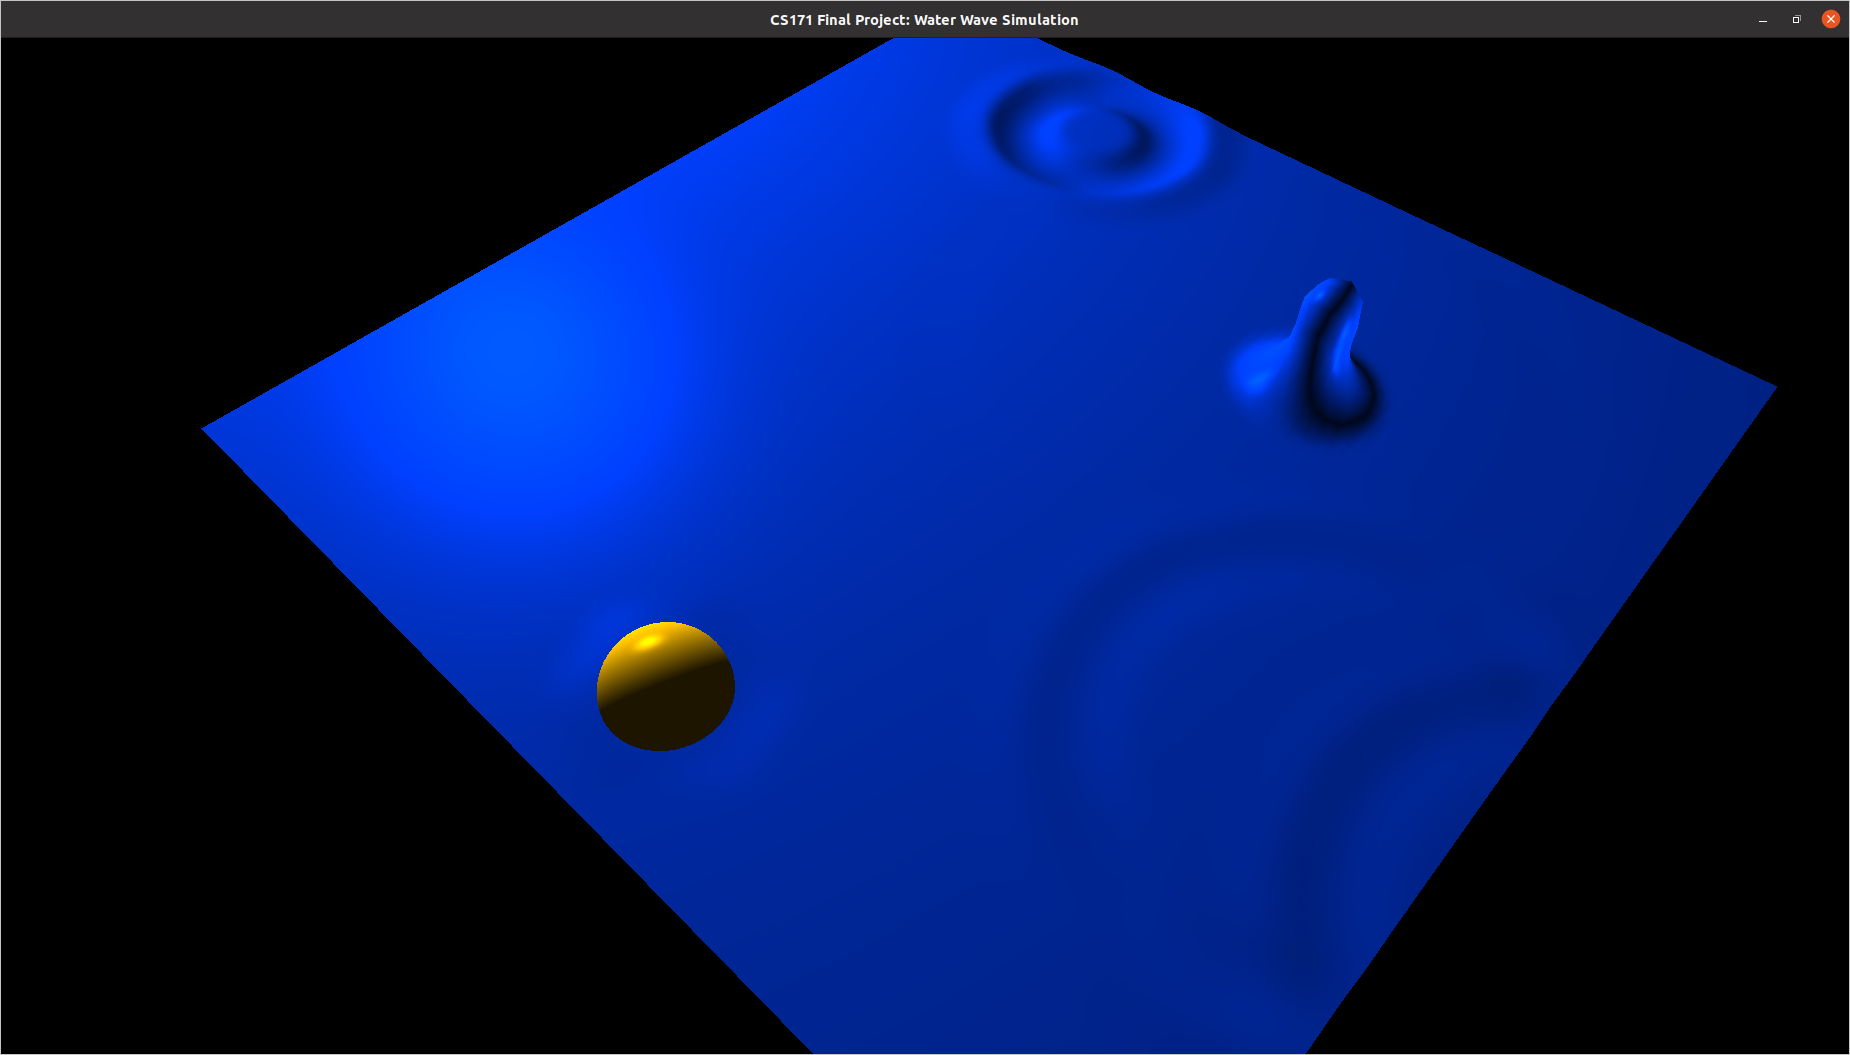
\includegraphics[scale=0.1]{image/Suppliment 1.png}
    }
    \subfigure[]{
		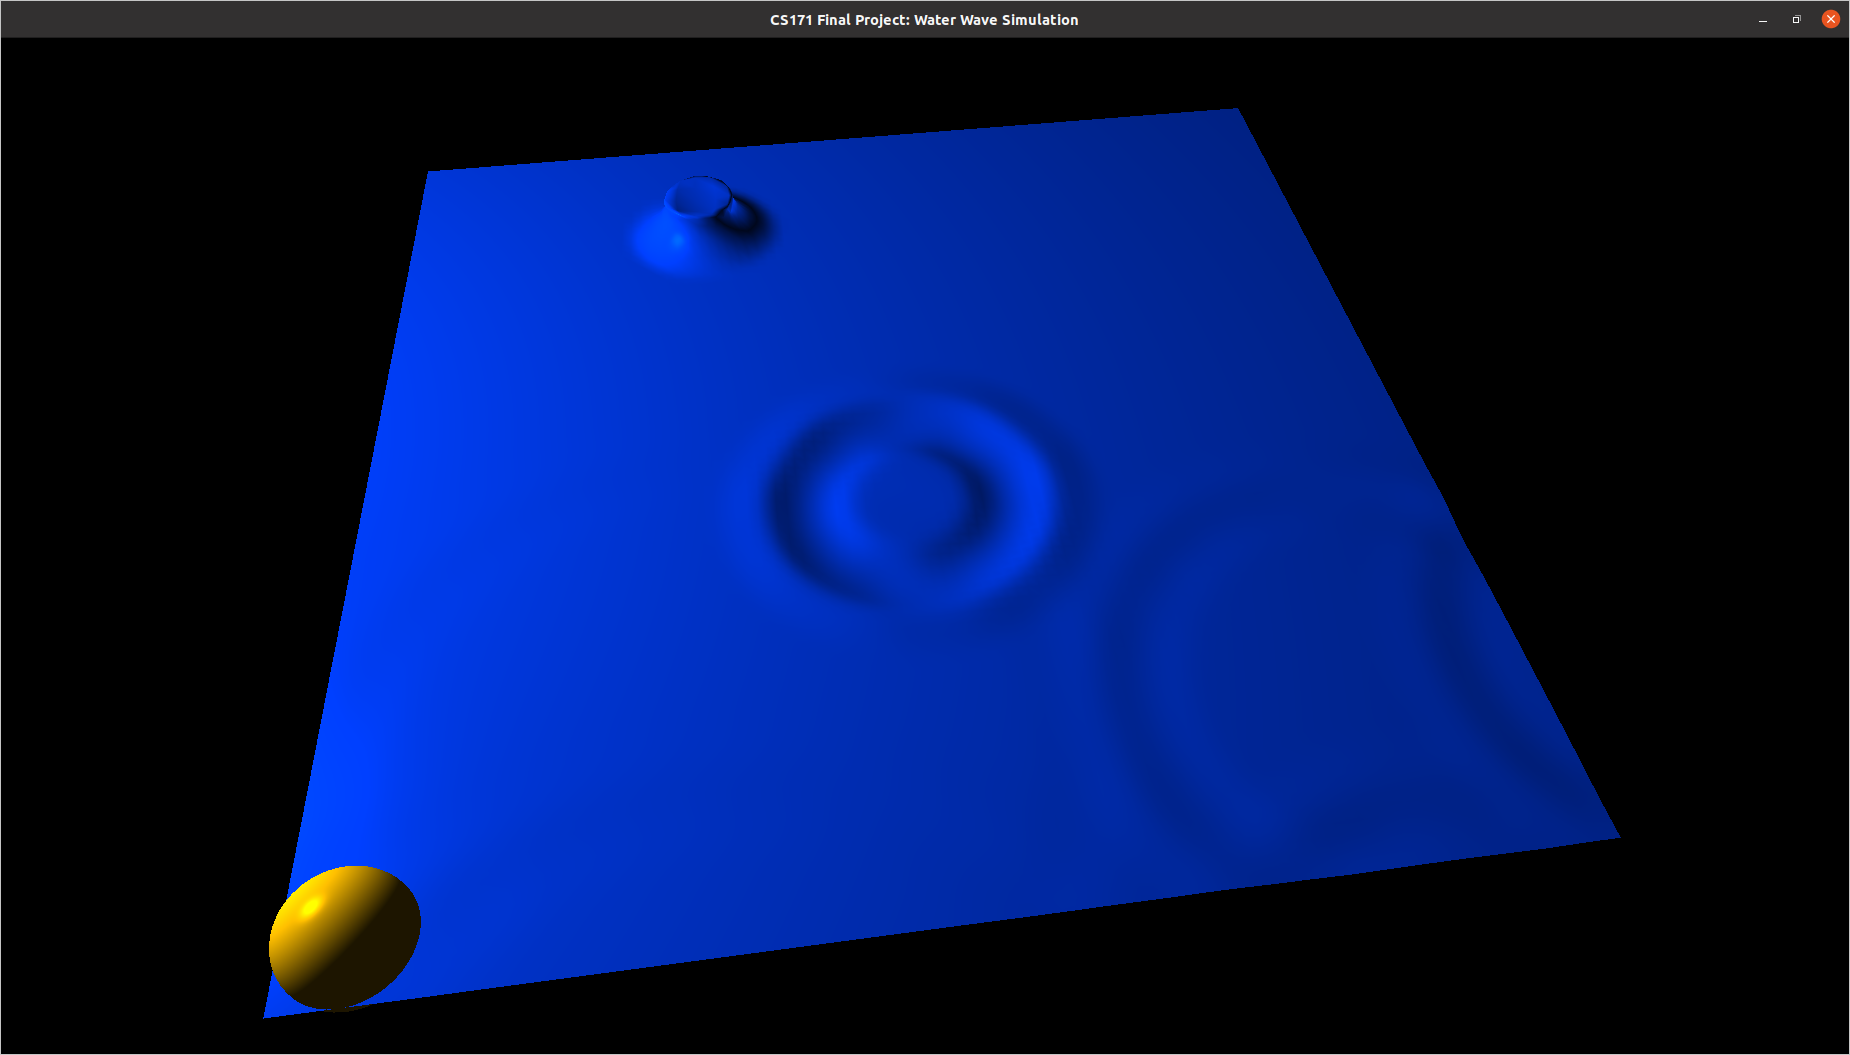
\includegraphics[scale=0.1]{image/Suppliment 2.png}
    }
	\caption{More supplementary results.}
\end{figure}
\section{Discussion}
The two main limitations of our project are as follows. 
The first one is fluid mesh interaction. Since the calculation of volume inside fluid for arbitrary mesh is very difficult for us and the time efficiency is not enough to traverse all triangle face in arbitrary mesh, we just implement the fluid-sphere interaction, where the sphere is seen as a whole. 
The other one is the low time efficiency, when the number of wave particles reaches a big number, our method will be very slow, the main cause is that when we render the height field, we will traverse all wave particles for every water vertex to calculate the vertical and horizontal components, which need $O(N^2)$ time complexity, so if we want to keep real time rendering, the number of all wave particles will have a strict limitation. 

For work division of our team, all the two team members in our group have taken part in all the work in this final project, including the research on the work to be realized and repeated, the coding part, the writing of the report and the preparation of the presentation. 
To be more specific, Yifan Qin is mainly in charge of the coding part of the final project and Yan Zeng helps in the implementation of the final project. 
For the report and presentation, Yan Zeng takes the initiative and Yifan Qin offers help.

\bibliographystyle{acm}
\bibliography{ref}

\end{document}
